\documentclass[aspectratio=169,11pt]{beamer}

\usetheme{Madrid}
\usecolortheme{default}
\setbeamertemplate{navigation symbols}{}
\setbeamertemplate{footline}[frame number]

\usepackage{amsmath,amssymb}
\usepackage{graphicx}
\usepackage{tikz}
\usetikzlibrary{positioning,calc}
\usetikzlibrary{arrows.meta,decorations.pathmorphing}

\definecolor{RamRed}{RGB}{190,40,45}
\definecolor{RamBlue}{RGB}{30,90,180}
\definecolor{SoftGray}{RGB}{245,245,245}
\definecolor{DarkGray}{RGB}{70,70,70}
\definecolor{MapGreen}{RGB}{48,150,95}
\definecolor{MapGold}{RGB}{235,180,45}

\setbeamercolor{title}{fg=DarkGray}
\setbeamercolor{frametitle}{fg=white,bg=RamBlue}
\setbeamercolor{structure}{fg=RamBlue}

\tikzset{
  v/.style={circle,draw=black,fill=white,inner sep=1.8pt},
  edge/.style={draw=RamBlue,line width=1.25pt},
  topic/.style={draw=black!30,fill=SoftGray,rounded corners=5pt,inner sep=7pt,
    text width=5.8cm,minimum height=1.65cm,align=left},
}


\usepackage{booktabs}
\tikzset{dot/.style={circle,fill=black,inner sep=2pt}, lab/.style={circle,draw=black,fill=white,inner sep=2pt,minimum size=6mm,font=\small},selected/.style={draw=RamRed,line width=2pt}}

\newcommand{\Def}[2]{\begin{block}{#1}#2\end{block}}
\newcommand{\Thm}[2]{\begin{block}{#1}#2\end{block}}
\renewcommand{\Proof}[1]{\begin{block}{Proof}\normalsize #1\end{block}}
\newcommand{\Question}[1]{\begin{block}{Question}#1\end{block}}
\renewcommand{\Example}[1]{\begin{block}{Example}#1\end{block}}
\newcommand{\fall}[2]{#1^{\underline{#2}}}
\newcommand{\rise}[2]{#1^{\overline{#2}}}
\newcommand{\stir}[2]{\left\{\begin{matrix}#1\\#2\end{matrix}\right\}}
\newcommand{\cyc}[2]{\left[\begin{matrix}#1\\#2\end{matrix}\right]}
\newcommand{\eul}[2]{\left\langle\begin{matrix}#1\\#2\end{matrix}\right\rangle}
\newcommand{\coef}[2]{[#1^{#2}]}
\newcommand{\gap}{\par\medskip}

\title{Multinomial Coefficients}
\author{Jeremy Quastel}\date{}\begin{document}
\begin{frame}[plain]\begin{center}{\Huge\bfseries Multinomial Coefficients}\par\vspace{.25cm}{\Large Section 2.3}\par\vspace{.15cm}{\large Harris--Hirst--Mossinghoff, \emph{Combinatorics and Graph Theory}}\par\vspace{.1cm}\resizebox{!}{2.7cm}{\begin{tikzpicture}[x=.65cm]\foreach \i in {1,2,4,5,6,8,9}{\node at (\i,0){$\star$};}\draw[thick](3,-.35)--(3,.35);\draw[thick](7,-.35)--(7,.35);\node at (5,-.8){$2+3+2=7$};\end{tikzpicture}}\par\vspace{.25cm}Jeremy Quastel\end{center}\end{frame}
\begin{frame}[plain]\large \begin{center}{\Huge\bfseries Today\textquotesingle s lecture}\par\vspace{.5cm}\end{center}\begin{columns}[c,onlytextwidth]\begin{column}{.48\textwidth}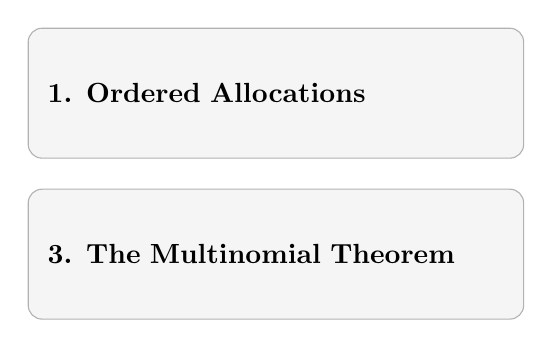
\begin{tikzpicture}\node[topic](a){\textbf{1. Ordered Allocations}};\node[topic,below=.38cm of a]{\textbf{3. The Multinomial Theorem}};\end{tikzpicture}\end{column}\begin{column}{.48\textwidth}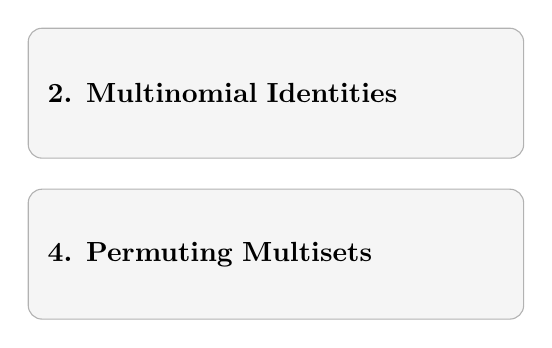
\begin{tikzpicture}\node[topic](a){\textbf{2. Multinomial Identities}};\node[topic,below=.38cm of a]{\textbf{4. Permuting Multisets}};\end{tikzpicture}\end{column}\end{columns}\end{frame}
\begin{frame}{More than two classes}
\large
\Question{How many ways can $10$ distinct students be assigned to three labeled groups of sizes $4,3,3$?}
\gap Choose the first group, then the second, then the third:
\[\binom{10}4\binom63\binom33=\frac{10!}{4!3!3!}=4200.\]
\end{frame}
\begin{frame}{Multinomial coefficients}
\large
\Def{Definition}{If $n_1+\cdots+n_r=n$ with each $n_i\geq0$, define
\[\binom n{n_1,n_2,\ldots,n_r}=\frac{n!}{n_1!n_2!\cdots n_r!}.\]}
\gap This counts allocations of $n$ distinct objects to $r$ labeled boxes with specified occupancies $n_1,\ldots,n_r$.
\end{frame}
\begin{frame}{Choosing the boxes successively}
\large
\[\binom n{n_1}\binom{n-n_1}{n_2}\cdots
\binom{n-n_1-\cdots-n_{r-1}}{n_r}
=\binom n{n_1,\ldots,n_r}.\]
\gap Factorials cancel in the product. Every allocation appears exactly once.
\end{frame}
\begin{frame}{A permutation proof}
\large
\Proof{Order all $n$ objects, then cut the ordering into consecutive blocks of sizes $n_1,\ldots,n_r$. There are $n!$ orderings.\gap Permuting objects within a block does not change the allocation. Each allocation arises from $n_1!\cdots n_r!$ orderings. Divide by this common multiplicity.}
\end{frame}
\begin{frame}{Labeled and unlabeled groups}
\large
\Question{How many ways can six people be divided into three unlabeled pairs?}
\gap Labeled pairs give $6!/(2!)^3=90$ allocations. Each unlabeled pairing has $3!$ labelings, so the answer is
\[\frac{6!}{(2!)^3 3!}=15.\]
\gap Dividing by $3!$ is justified because all three groups have the same required size.
\end{frame}
\begin{frame}{Symmetry}
\large
\[\binom n{n_1,n_2,\ldots,n_r}
=\binom n{n_{\sigma(1)},n_{\sigma(2)},\ldots,n_{\sigma(r)}}\]
for every permutation $\sigma$ of the box labels.
\gap Relabeling the boxes is a bijection between the corresponding allocations.
\end{frame}
\begin{frame}{A multinomial recurrence}
\large
\Thm{Identity}{If $n_1+\cdots+n_r=n\geq1$, then
\[\binom n{n_1,\ldots,n_r}
=\sum_{i:n_i>0}\binom{n-1}{n_1,\ldots,n_i-1,\ldots,n_r}.\]}
\Proof{Fix one object and distinguish the box containing it. Then allocate the other $n-1$ objects.}
\end{frame}
\begin{frame}{The multinomial theorem}
\large
\Thm{Theorem}{For every nonnegative integer $n$,
\[(x_1+\cdots+x_r)^n=
\sum_{n_1+\cdots+n_r=n}\binom n{n_1,\ldots,n_r}x_1^{n_1}\cdots x_r^{n_r},\]
where the sum is over nonnegative integers $n_1,\ldots,n_r$.}
\end{frame}
\begin{frame}{Proof of the multinomial theorem}
\large
\Proof{In the product of $n$ factors $(x_1+\cdots+x_r)$, assign each factor to the term chosen from it.\gap To obtain $x_1^{n_1}\cdots x_r^{n_r}$, assign $n_i$ factors to $x_i$ for each $i$. The number of assignments is the multinomial coefficient.}
\end{frame}
\begin{frame}{An expansion}
\large
\normalsize
\begin{align*}
(x+y+z)^3={}&x^3+y^3+z^3\\
&+3x^2y+3x^2z+3y^2x+3y^2z+3z^2x+3z^2y\\
&+6xyz.
\end{align*}
\gap The coefficients add to $3^3=27$.
\gap The coefficient of $xyz$ is $\binom3{1,1,1}=6$.
\end{frame}
\begin{frame}{Coefficient extraction}
\large
\Question{Find the coefficient of $x^2y^3z$ in $(2x-y+3z)^6$.}
\gap Choose two $2x$ terms, three $-y$ terms, and one $3z$ term:
\[\binom6{2,3,1}2^2(-1)^3 3=-720.\]
\end{frame}
\begin{frame}{Summing multinomial coefficients}
\large
\Thm{Identity}{\[\sum_{n_1+\cdots+n_r=n}\binom n{n_1,\ldots,n_r}=r^n.\]}
\Proof{Set every variable equal to $1$ in the multinomial theorem. Alternatively, count all assignments of $n$ distinct objects to $r$ labeled boxes by their occupancies.}
\end{frame}
\begin{frame}{Words with prescribed multiplicities}
\large
\Thm{Theorem}{The number of words containing $n_i$ copies of symbol $i$, for $i=1,\ldots,r$, is
\[\frac{(n_1+\cdots+n_r)!}{n_1!\cdots n_r!}.\]}
\gap Choose which positions receive each symbol. Equal symbols are indistinguishable.
\end{frame}
\begin{frame}{Rearranging MISSISSIPPI}
\large
\Example{The word MISSISSIPPI has $11$ letters: one M, four I's, four S's, and two P's.}
\gap Its distinct rearrangements number
\[\frac{11!}{1!4!4!2!}=34,650.\]
\end{frame}
\begin{frame}{Rearranging BOOKKEEPER}
\large
\Example{BOOKKEEPER has $10$ letters: two O's, two K's, three E's, and one each of B, P, R.}
\[\frac{10!}{2!2!3!}=151,200.\]
\gap Counting the multiplicities correctly comes before applying the formula.
\end{frame}
\begin{frame}{Multidimensional lattice paths}
\large
\Question{How many paths from $(0,0,0)$ to $(a,b,c)$ take positive unit steps along coordinate axes?}
\gap Encode a path by a word with $a$ X's, $b$ Y's, and $c$ Z's. Therefore the answer is
\[\binom{a+b+c}{a,b,c}.\]
\end{frame}
\begin{frame}{Using only some of a multiset}
\large
\Question{How many three-letter words can be made from $\{a,a,a,b,b,c\}$ without exceeding the available multiplicities?}
\gap A single multinomial coefficient does not apply: different words can use different numbers of each letter.
\gap Split into cases according to the multiplicity pattern.
\end{frame}
\begin{frame}{Partial words: the cases}
\large
\normalsize
\begin{center}\renewcommand{\arraystretch}{1.4}
\begin{tabular}{ccl}
Pattern & Number & Explanation\\\hline
Three equal & $1$ & Only $aaa$\\
Two equal, one different & $4\cdot3=12$ & $aab,aac,bba,bbc$, each reordered\\
All different & $3!=6$ & Rearrangements of $abc$
\end{tabular}\end{center}
\gap Total: $1+12+6=19$.
\end{frame}
\begin{frame}{The general formula for partial words}
\large
\Thm{Formula}{From a multiset having $m_i$ copies of symbol $i$, the number of words of length $k$ is
\[\sum_{\substack{n_1+\cdots+n_r=k\\0\leq n_i\leq m_i}}
\frac{k!}{n_1!\cdots n_r!}.\]}
\gap First specify the multiplicities used; then count the words with those multiplicities.
\end{frame}
\begin{frame}{A distinguished object in a box}
\large
\Thm{Identity}{When $n_i>0$,
\[n_i\binom n{n_1,\ldots,n_r}
=n\binom{n-1}{n_1,\ldots,n_i-1,\ldots,n_r}.\]}
\Proof{Count an allocation together with a distinguished object in box $i$. Choose the allocation first, or choose the distinguished object first.}
\end{frame}
\begin{frame}{Practice}
\large
\Question{How many words have four A's, three B's, and two C's, with the two C's adjacent?}
\gap Treat the adjacent C's as one block.
\end{frame}
\begin{frame}{Practice: solution}
\large
\Proof{Replace CC by a single new symbol. We now arrange eight objects: four A's, three B's, and one CC block. Hence
\[\frac{8!}{4!3!}=280.\]
Expanding the block is a bijection back to the required words.}
\end{frame}
\begin{frame}{Summary}
\large
\begin{itemize}
\item Multinomial coefficients count prescribed allocations into labeled boxes.
\item They are the coefficients of powers of sums with several terms.
\item The same formula counts words with repeated symbols.
\item Partial words require a sum over the multiplicities actually used.
\end{itemize}
\end{frame}
\begin{frame}{Next time: The Pigeonhole Principle}\begin{center}{\Huge The Pigeonhole Principle}\end{center}\end{frame}
\end{document}